\documentclass[11pt]{article}

% some definitions for the title page
\newcommand{\reporttitle}{Convolutional Neural Networks and Curse of Dimensionality}
\newcommand{\reportdescription}{Explains the concept of curse of dimensionality and refresher on CNN architectures}

% load some definitions and default packages
%---------------------------------------------------------------------------
%	PACKAGES AND OTHER DOCUMENT CONFIGURATIONS
%---------------------------------------------------------------------------

\usepackage[twoside]{fancyhdr}
\usepackage{csquotes}

\usepackage[a4paper,hmargin=2.0cm,vmargin=1.0cm,includeheadfoot]{geometry}
% \usepackage{natbib} % for bibliography
\usepackage{biblatex}
\usepackage{tabularx,longtable,multirow,subfigure,caption}%hangcaption
\usepackage{fancyhdr} % page layout
\usepackage{url} % URLs
\usepackage[english]{babel}
\usepackage{graphicx}
\usepackage{rotating}
\usepackage{dsfont}
\usepackage{epstopdf} % automatically replace .eps with .pdf in graphics
% \usepackage{backref} % needed for citations
\usepackage{array}
\usepackage{latexsym}
\usepackage[pdftex,hypertexnames=false,colorlinks]{hyperref} % provide links in pdf (had pagebackref)
\usepackage{booktabs}
\usepackage{wrapfig}
\usepackage{caption}  % Required for \captionof
\usepackage{float} % for H option in figures
\usepackage{amssymb}
\usepackage{amsmath}
\usepackage{amsthm}
\usepackage{mathtools} % for 'dcases*' env.
\usepackage[nottoc]{tocbibind}

%%% Default fonts
\renewcommand*{\rmdefault}{bch}
\renewcommand*{\ttdefault}{cmtt}

%%% Default settings (page layout)
\setlength{\parindent}{0em}  % indentation of paragraph
\setlength{\parskip}{.3em}
\setlength{\itemsep}{0.mm}

\setlength{\headheight}{14.5pt}
\pagestyle{fancy}

\fancyfoot[ER,OL]{\thepage}%Page no. in the left on odd pages and on right on even pages

\fancyfoot[OC,EC]{\sffamily }
\renewcommand{\headrulewidth}{0.1pt}
\renewcommand{\footrulewidth}{0.1pt}
\captionsetup{margin=10pt,font=small,labelfont=bf}

% LISTINGS ammendments
\usepackage{listings}
\usepackage{color}

\definecolor{mygreen}{rgb}{0,0.6,0}
\definecolor{mygray}{rgb}{0.5,0.5,0.5}
\definecolor{mymauve}{rgb}{0.58,0,0.82}

\lstset{ 
  postbreak=\mbox{\textcolor{red}{$\hookrightarrow$}\space},
  backgroundcolor=\color{white},   % choose the background color; you must add \usepackage{color} or \usepackage{xcolor}; should come as last argument
  basicstyle=\footnotesize,        % the size of the fonts that are used for the code
  breakatwhitespace=false,         % sets if automatic breaks should only happen at whitespace
  breaklines=true,                 % sets automatic line breaking
  captionpos=b,                    % sets the caption-position to bottom
  commentstyle=\color{mygreen},    % comment style
%   deletekeywords={...},            % if you want to delete keywords from the given language
%   escapeinside={\%*}{*)},          % if you want to add LaTeX within your code
  extendedchars=true,              % lets you use non-ASCII characters; for 8-bits encodings only, does not work with UTF-8
  firstnumber=1,                % start line enumeration with line 1000
  frame=single,	                   % adds a frame around the code
  keepspaces=true,                 % keeps spaces in text, useful for keeping indentation of code (possibly needs columns=flexible)
  columns=fullflexible,
  keywordstyle=\color{blue},       % keyword style
  language=python,                 % the language of the code
  % morekeywords={*,...},            % if you want to add more keywords to the set
  numbers=left,                    % where to put the line-numbers; possible values are (none, left, right)
  numbersep=5pt,                   % how far the line-numbers are from the code
  numberstyle=\tiny\color{mygray}, % the style that is used for the line-numbers
  rulecolor=\color{black},         % if not set, the frame-color may be changed on line-breaks within not-black text (e.g. comments (green here))
  showspaces=false,                % show spaces everywhere adding particular underscores; it overrides 'showstringspaces'
  showstringspaces=false,          % underline spaces within strings only
  showtabs=false,                  % show tabs within strings adding particular underscores
  stepnumber=1,                    % the step between two line-numbers. If it's 1, each line will be numbered
  stringstyle=\color{mymauve},     % string literal style
  tabsize=2,	                   % sets default tabsize to 2 spaces
  title=\lstname% show the filename of files included with \lstinputlisting; also try caption instead of title
}

% Here, you can define your own macros. Some examples are given below.

\newcommand{\R}[0]{\mathds{R}} % real numbers
\newcommand{\Z}[0]{\mathds{Z}} % integers
\newcommand{\N}[0]{\mathds{N}} % natural numbers
\newcommand{\C}[0]{\mathds{C}} % complex numbers
\renewcommand{\vec}[1]{{\boldsymbol{{#1}}}} % vector
\newcommand{\mat}[1]{{\boldsymbol{{#1}}}} % matrix


\bibliography{bibliography}

\begin{document}

% Include the title page
\begin{titlepage}

    \newcommand{\HRule}{\rule{\linewidth}{0.5mm}} % Defines a new command for the horizontal lines, change thickness here
    
    \center % Center everything on the page
     
    %------------------------------------------------------------------------
    %	HEADING SECTIONS
    %------------------------------------------------------------------------
    
    \textsc{\Large Department of Computing}\\[0.5cm] 
    \textsc{\large Imperial College of Science, Technology and Medicine}\\[0.5cm] 
    
    %------------------------------------------------------------------------
    %	TITLE SECTION
    %------------------------------------------------------------------------
    
    \HRule \\[0.4cm]
    { \huge \bfseries \reporttitle}\\ % Title of your document
    \HRule \\[0.4cm]

    \textit{\reportdescription}
    
    \vspace{2em}

    %------------------------------------------------------------------------
    %	AUTHOR SECTION
    %------------------------------------------------------------------------
    
    \large \emph{Author: Anton Zhitomirskiy}

    \vspace{1em}

    \global\let\newpagegood\newpage
    \global\let\newpage\relax
    
\end{titlepage}

\global\let\newpage\newpagegood

\tableofcontents

\clearpage

\section{Learning System}

\subsection{Fundamental components}

The learning framework consists of 3 fundamental components:

\begin{enumerate}
    \item Feature Extractor: responsible for capturing the hierarchical patterns in the data - edges, textures, and more complex shapes. It is what allows the network to `understand' what it's looking at.
    \item Task-specific Head: tailored to the problem we're trying to solve. Takes the rich features extracted by the feature extractor and maps them to the specific task at hand.
    \item Parameter Optimization: using algorithms like stochastic gradient descent, the model fine-tunes its parameters to minimize a loss function.
\end{enumerate}

\subsection{Challenges in image analysis}

\begin{enumerate}
    \item dealing with the sheer complexity and size of image data
    \item Traditional neural networks, however, don't have an innate understanding of the spatial hierarchies that are present in image data
    \item translation invariance. For instance, if a traditional neural network is trained to recognize a cat in the bottom-left corner of an image, it may not easily recognize that same cat if it appears in the top-right corner
    \item over-fitting - The risk amplifies because of the high number of parameters involved in these models
\end{enumerate}

\subsection{Universal Approximator}

``The Universal Approximation Theorem tells us that Neural Networks has a kind of universality i.e. no matter what f(x) is, there is a network that can approximately approach the result and do the job! This result holds for any number of inputs and outputs''~\cite{towardsdatascienceNeuralNetworks}

\begin{theorem}[Universal Approximator]\label{theorem:universal-approximator}
    Let $\phi(\cdot)$ be a non-constant, bounded\footnote{It has been shown that it even works with \href{https://edstem.org/us/courses/46843/discussion/4124905}{unbounded}} and monotonically increasing function. For any $\epsilon > 0$ and any continuous function defined on a compact subset of $\mathbb{R}^m$, there exists an integer $N$, real constants $v_i b_i \in \mathbb{R}$ and real vectors $w_i \in \mathbb{R}$ where $i=1, \ldots N$ such that:

    \begin{equation}
        F(\vec{x})=\sum^N_{i=1}v_i\phi(\vec{w}_i^T\vec{x}+b_i) \quad \text{with } |F(\vec{x}) - f(\vec{x})| < \epsilon
    \end{equation}

    We assume that $\phi$ is a sensible activation function, like the sigmoid or ReLU.
\end{theorem}

\subsubsection{Problems}

\begin{enumerate}
    \item $\epsilon$ can be very large in practice, making the approximation less useful.
    \item Curse of dimensionality\footnote{Section~\ref{sect:curse-of-dimensionality}}, where the number of computational and spatial complexity increases exponentially with the number of dimensions.
\end{enumerate}

\subsubsection{Solution}

To tackle these issues, the typical solution is to break up the problem into many smaller problems, which is essentially what multiple layers in deep neural networks do. This hierarchical decomposition allows us to learn complex functions more effectively.

\section{Curse of Dimensionality}\label{sect:curse-of-dimensionality}

\begin{definition}[Sample Explosion]\label{def:sample-explosion}
    As the number of features or dimensions grows, the amount of data we need to generalize accurately grows exponentially.

    To approximate a (Lipschitz) continuous function $f: \mathbb{R}^d \rightarrow \mathbb{R}$ with $\epsilon$ accuracy one needs $O(\epsilon^{-d})$ samples.
\end{definition}

We also find that as the number of dimensions increases, the performance of a model increases and falls after a point~\cite{visiondummyCurseDimensionality}.

\begin{figure}[H]
    \centering
    \subfigure{\includegraphics*[width=.32\linewidth]{figures/3d-split.png}}
    \subfigure{\includegraphics*[width=.32\linewidth]{figures/3d-on-2d-split.png}}
    \subfigure{\includegraphics*[width=.32\linewidth]{figures/2d-split.png}}
    \caption{Demonstration of overfitting when introducing more features~\cite{visiondummyCurseDimensionality}}\label{fig:more-features-overfitting}
\end{figure}

Adding the third dimension in Figure~\ref{fig:more-features-overfitting} to obtain perfect classification results, simply corresponds to using a complicated non-linear classifier in the lower dimensional feature space. If we would keep adding features, the dimensionality of the feature space grows, and becomes sparser and sparser. Due to this sparsity, it becomes much more easy to find a separable hyperplane because the likelihood that a training sample lies on the wrong side of the best hyperplane becomes infinitely small when the number of features becomes infinitely large. This concept is called overfitting and is a direct result of the curse of dimensionality.

\subsection{Sample Explosion}

If we have a function $f$ as in Theorem~\ref{theorem:universal-approximator} and we want to approximate this function with a specific level of accuracy, denoted as $\epsilon$, then the number of sampels required to achieve this level of accuracy $\epsilon$ grows exponentially with dimension $d$ as in Definition~\ref{def:sample-explosion}.

\subsection{Sparseness}

\begin{figure}[H]
    \centering
    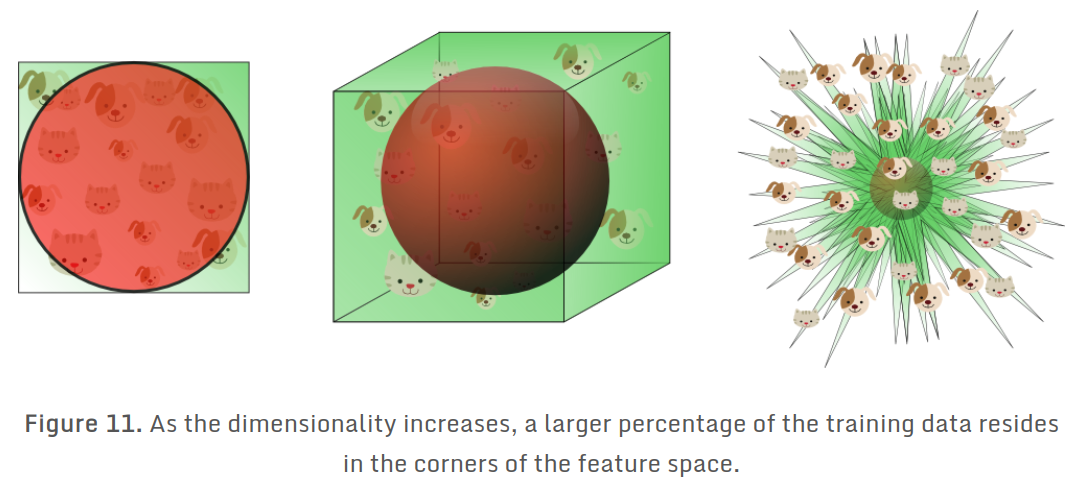
\includegraphics[width=.8\linewidth]{figures/edgeness-of-high-dimensions.png}
    \caption{Sparseness of data as you add more dimensions. The data points sit around the edges, rather than in the center~\cite{visiondummyCurseDimensionality}}\label{fig:edgeness-of-data}
\end{figure}

The more features we use, the more sparse the data becomes such that accurate estimation of the classifier’s parameters (i.e. its decision boundaries) becomes more difficult. Another effect of the curse of dimensionality, is that this sparseness is not uniformly distributed over the search space. In fact, data around the origin (at the center of the hypercube) is much more sparse than data in the corners of the search space.~\cite{visiondummyCurseDimensionality}.

Consider a 1D space; perhaps you're trying to approximate a line. If you need 10 samples for $\epsilon$-level accuracy in 1D, you'll need 100 8samples in 2D, and potentially 1,000 in 3D. The sample requirement explodes as dimensions increase, making the task computationally burdensome.

\subsubsection{Math}

Intuition taken from slides and~\cite{stackexchangeMathematicalDemonstration}.

\begin{enumerate}
    \item Suppose you have a n-dimensional shape. It is described by a set of $n$ vectors. If we want to create a proportionately smaller vector by factor $\alpha$ then we multiply by $\alpha$.
    \item Comparing the volume in the case of the 3-dimensional shape:
          \begin{align}
              V^3_{original} & =Width\times Height\times Length                                                                     \\
              V^3_{interior} & =\alpha Width\times \alpha Height\times \alpha Length                                                \\
                             & = \alpha^3 V_{original} \Rightarrow V^n_{interior} = \alpha^n V_{original}                           \\
              V^3_{rind}     & = (1-\alpha) Width\times (1-\alpha) Height\times (1-\alpha) Length\label{equ:rind-vs-interror-alpha} \\
                             & = (1-\alpha^3) V_{original}  \\ 
              \Rightarrow V^n_{rind}  & = (1-\alpha^n) V_{original}
          \end{align}
    \item The volume of the rind relative to the original volume therefore is
          \begin{align}
              \frac{V_{rind}}{V_{original}} = 1 - \alpha^n
          \end{align}
    \item We can define the rate of change of $\alpha$ relative to the ratio above as
          \begin{align}
              \frac{d (1 - \alpha^n)}{d\alpha} = -n\alpha^{n-1} \iff d(1-\alpha^n) = -n\alpha^{n-1}d\alpha\label{eq:rate-of-growth-alpha}
          \end{align}
    \item From Equation~\ref{eq:rate-of-growth-alpha} this shows that the volume of the rind initially grows much faster, n times faster than the rate at which the object is being shrunk (when $\alpha=1$ and $d\alpha < 0$ then $d(1-\alpha^n)=n|d\alpha|$)
    \item in higher dimensions, relatively tiny changes in distance translate to much larger changes in volume.
    \item In higher dimensions, minuscule changes in distance can lead to vast changes in volume. For machine learning practitioners, this has massive implications on data distribution, sampling, and model generalizability.
\end{enumerate}

We can find, for the general case, what the volume ratio would be to find 50\% of the data as follows:

\begin{enumerate}
    \item $\alpha^n = 0.5$ then $\alpha = 2^{-1/n} \approx 1 - 0.7 / n$
    \item From this, we have a formula to see how much we ought to shrink the object by such that 50\% of the data will be split amongst the rind and internal volume.
    \item E.g. in the 2-d case: $\alpha = 1 - 0.35$. Therefore, from the outer edges, $1 - \alpha = 0.35$ (We do $1 - \alpha$ as we needed to in Equation~\ref{equ:rind-vs-interror-alpha}).

          $0.35/2$ describes `cutting from both sides' so 0.18 of its diameter from the boundary will contain 50\% of the volume.
    \item For large dimensions, the half-length is very close to 1: $n=350$ gives 98\% - thus expect half of any 350-dimensional shape's volume to lie within 1\% of its diameter from its boundary.
\end{enumerate}

Therefore, without strong clustering, in higher dimensions n we can expect most Euclidean distances between observations in a dataset to be very nearly the same and to be very close to the diameter of the region in which they are enclosed. ``Very close'' means on the order of 1/n~\cite{stackexchangeMathematicalDemonstration}.

\subsection{Practical Meaning}

\begin{figure}[H]
    \centering
    \includegraphics*[width=.4\linewidth]{figures/hypersphere.png}
    \caption{As you increase dimensions the total volume of `useful' data is way smaller}
\end{figure}

The core takeaway is that as we go from 2D to 3D to even higher dimensions, the volume of the hypersphere starts to shrink significantly, becoming almost negligible compared to the volume of the hypercube.

This has a profound implication for machine learning: as the dimensionality of our feature space increases, most of our data points will reside in the corners of the hypercube.

Infact, as shown in Figure~\ref{fig:edgeness-of-data} the higher dimensions you have the higher probability that a data-point will sit in its own distinct corner in the hypercube. The distance between the corner will be equal. If we roll the high dimensional enclosing hypercubes into a n-dimensional torus, and we plot the distance between samples, we see that distances between points become approximately equal.

\begin{figure}[H]
    \centering
    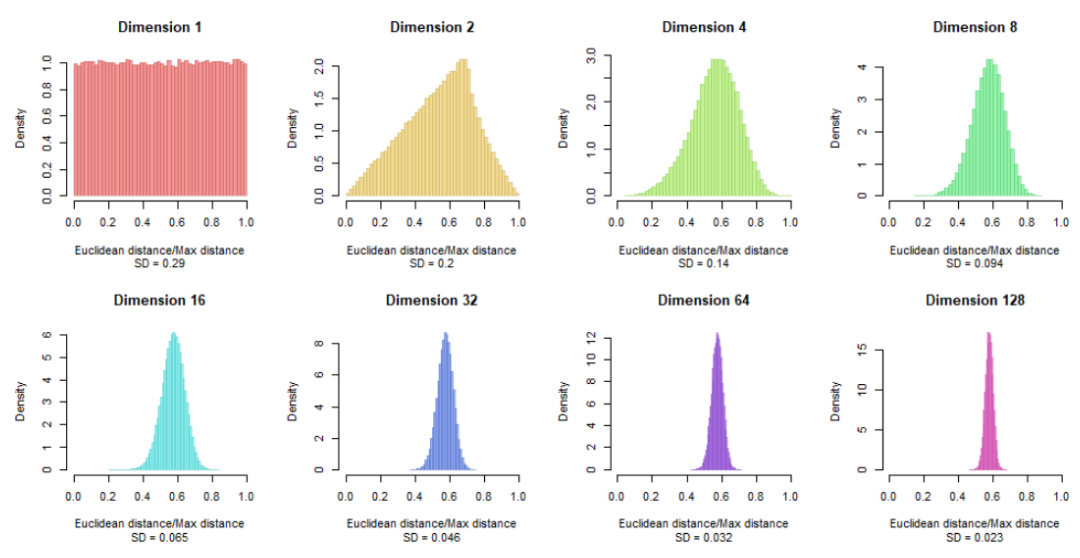
\includegraphics[width=.6\textwidth]{figures/distnace-between-points.png}
\end{figure}

\section{Invariance and Equivariance}

\begin{definition}[Shift Invariance]\label{def:shift-invariance}
    describes a system's unchanging response when the input is shifted. For example, some classifier $f$ and shift operator $S_v$, $f(\vec{x})=f(S_v\vec{x})$
\end{definition}

To put it simply, invariance is about stability. When we talk about invariance, what we mean is that no matter how the input is transformed, the output should remain constant.

Shift invariance is beneficial because it allows models to generalize better from their training data to new unseen data.

\begin{definition}[shift Equivariance]\label{def:shift-equivariance}
    applying the shift operator after the function yields the same results as applying the function after the shift. i.e. $S_v \circ f(\vec{x}) = f(\vec{x}) \circ S_v$
\end{definition}

Equivariance is about consistent transformation. In an equivariant system, the transformation applied to the input is exactly the same as the transformation applied to the output. For example, if we move an object within an image, the corresponding output should move in the same way.

\begin{figure}[H]
    \centering
    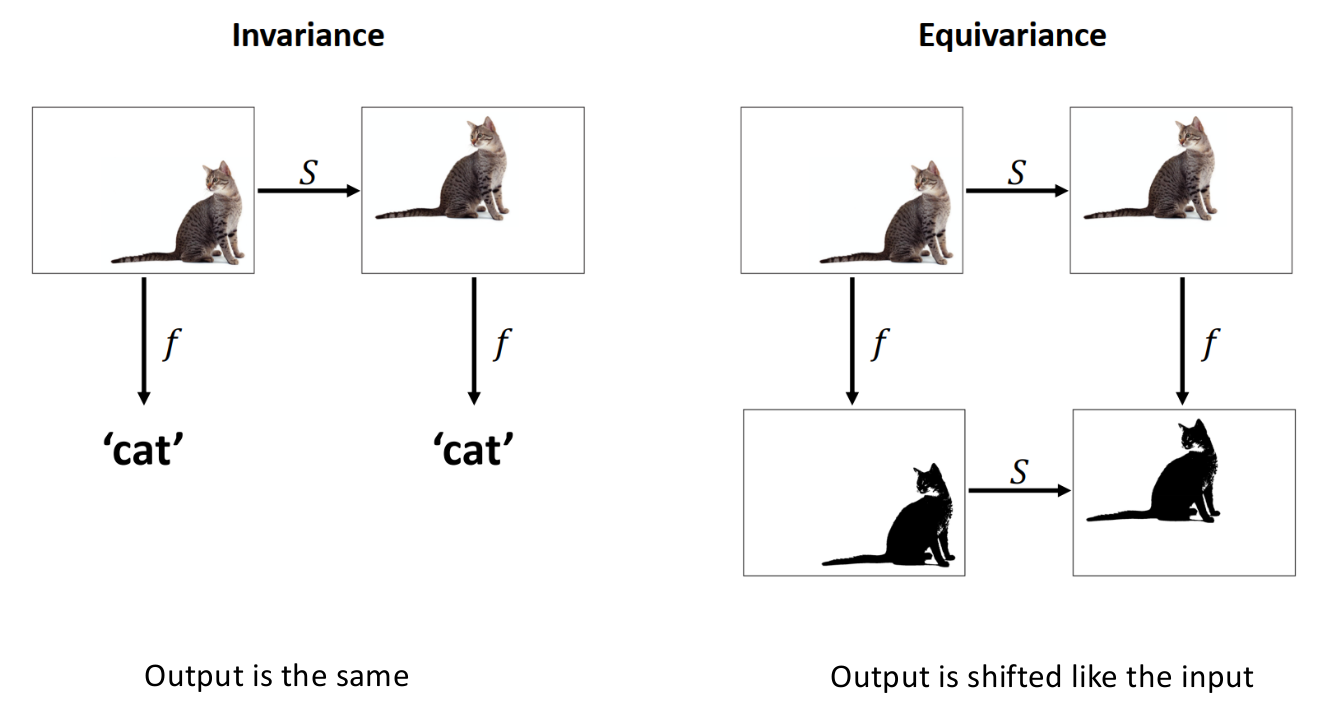
\includegraphics[width=.7\textwidth]{figures/equivariance-vs-invariance.png}
    \caption{Equivariance vs Invariance}
\end{figure}

\section{Inductive Bias/assumptions}

\subsection{Translation invariance}

A shift in the input should simply lead to a shift in the hidden representation in a predictable manner. The essence of what is being represented should not change simply because its location in the input space has changed.

\subsection{Locality}

we believe that we should not have to look very far away from any location (i,j) in order to glean relevant information to assess what  this area contains.

\subsection{Practical Application}

We can use a sliding window and come up with a correlation metric to see if a patch is on an image. The first principle tells us it doesn't matter where in the image the patch is located, the second means that operating under the assumption that lal the information needed to identify the person is found in a local neighborhood of pixels.

\section{Convolutions}

\subsection{Fully connected neural network}

\begin{figure}[H]
    \centering
    \subfigure{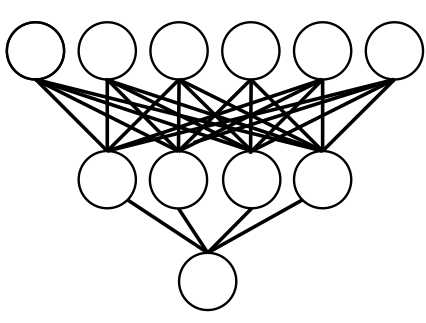
\includegraphics[width=0.3\textwidth]{figures/fully-convolutional-network-graph.png}}
    \subfigure{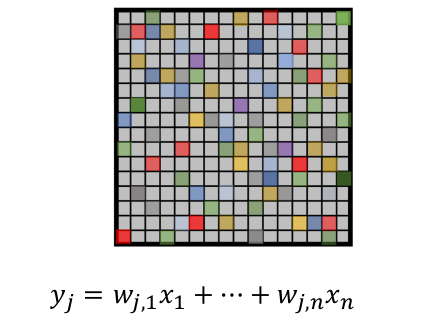
\includegraphics[width=0.3\textwidth]{figures/fully-convolutional-network-image.png}}
    \caption{Fully convolutional neural network}
\end{figure}

In a fully connected network, each input is connected to each node in the subsequent layer. This means that every single input feature influences every single neuron in the next layer. This is flexible, yet overfits and is computationally expensive.

For each node, the output would be a linear combination of all nodes in the layer before it. In an $n\times n$ matrix, then for a standard high-resolution image of 36 million elements, this will be too many parameters.

\subsection{Sparsely Connected neural networks }

\begin{figure}[H]
    \centering
    \subfigure{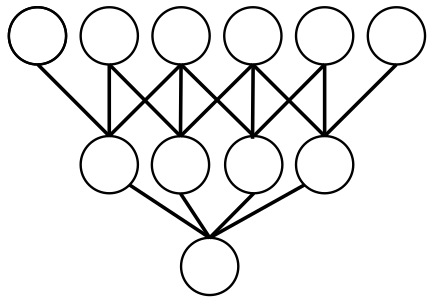
\includegraphics[width=0.3\textwidth]{figures/sparsley-convolutional-network-graph.png}}
    \subfigure{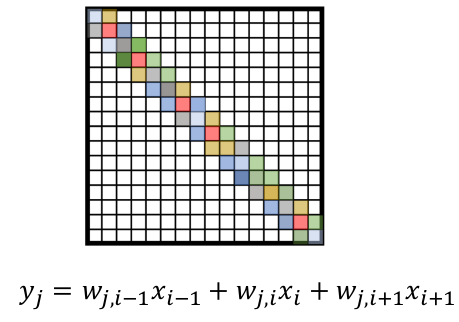
\includegraphics[width=0.3\textwidth]{figures/sparsley-convolutional-network-image.png}}
    \caption{Sparsely convolutional neural network}
\end{figure}

In this architecture, each input neuron is connected to only a small number k of hidden neurons, rather than to every neuron in the hidden layer. This reduces the amount parameters greatly, if we choose to connect to $k$ neurons, then size is $k\times n$.

\subsection{Weight Sharing neural networks }

\begin{figure}[H]
    \centering
    \subfigure{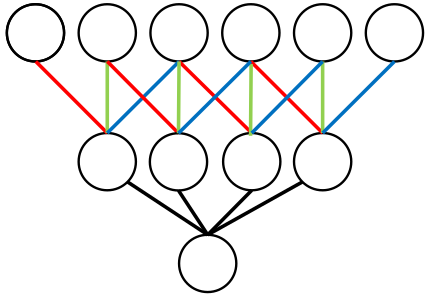
\includegraphics[width=0.3\textwidth]{figures/shared-convolutional-network-graph.png}}
    \subfigure{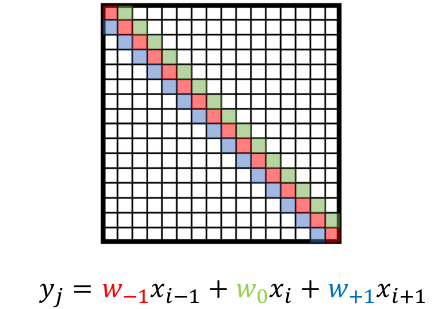
\includegraphics[width=0.3\textwidth]{figures/shared-convolutional-network-image.png}}
    \caption{Weight sharing convolutional neural network}
\end{figure}

The same weights $w_{-1},w_0,w_{+1}$ are reused for different input neurons. This is what we refer to as 'weight sharing.' It means that a subset of weights are identical, not just sparse. In other words, the same set of weights is used across multiple connections. This results in an even more dramatic reduction of parameters. For instance, if k=3, we only have 3 parameters that are shared. That's it, just 3 parameters, no matter the size of your input!

The image you see on the slide of a sparsely connected matrix should now look different to you: it's not just sparse; it's also sharing weights across its connections. This is one of the fundamental ideas that make convolutional neural networks so powerful and efficient.

\subsection{Convolution vs Correlation}

Both are essential operations in the realm of image processing and neural networks, but they have subtle differences.

Convolution involves flipping the kernel before performing the element-wise multiplication and sum, whereas correlation doesn't involve flipping. In other words, in convolution, we take the mirror image of the kernel across its central point before sliding it across the image. In correlation, the kernel is slid across the image as is, without any flipping.

\begin{definition}[Convolution (continuous)]
    \begin{equation}
        (f \ast g)(t) = \int^\infty_{-\infty} f(\tau)g(t-\tau) d\tau \quad for f,g:[0,\infty] \rightarrow \mathbb{R}
    \end{equation}
\end{definition}

This video has a great explanation~\cite{youtubeConvolutionsProbability}

\begin{definition}[Convolution (discrete)]
    \begin{equation}
        s_t = \sum_{a=-\infty}^{+\infty}u_a w_{t-a}
    \end{equation}
\end{definition}

\begin{definition}[Correlation]
    \begin{equation}
        (f \ast g)(t) = \int^\infty_{-\infty} f(\tau)g(t+\tau) d\tau \quad for f,g:[0,\infty] \rightarrow \mathbb{R}
    \end{equation}
\end{definition}

\subsubsection{Commutativity}

\begin{definition}[Commutativity of convolutions]
    \begin{align*}
        (f\ast g)(n)                                           &  & \text{starting point, what is the convoution at position n?} \\
        = \sum^\infty_{i=-\infty}f(i) \cdot g(n-i)             &  & \text{by convolution rule}                                   \\
        = \sum^{j=n-\infty}_{j=n-(-\infty)}f(n-j') \cdot g(j') &  & \text{substitute } j'=n-i                                    \\
        = \sum^{-\infty}_{j=\infty}f(n-j') \cdot g(j')         &  & \text{fix the bounds of the sum}                             \\
        = \sum^\infty_{j=-\infty}f(n-j') \cdot g(j')           &  & \text{commutivity of addition}                               \\
        = (g*f)(n)                                             &  & \text{apply convolution rule}
    \end{align*}
\end{definition}

\subsubsection{Associativity}

\begin{definition}[Associativity of convolutions]
    \begin{align*}
        ((f\ast g) \ast h)(n)                                                            &  & \text{starting point, what is the convoution at position n?}               \\
        = \sum^\infty_{i=-\infty}(f \ast g)(i) \cdot h(n-i)                              &  & \text{by convolution rule}                                                 \\
        = \sum^\infty_{i=-\infty}(\sum^\infty_{j=-\infty}f(j) \cdot g(i-j)) \cdot h[n-i] &  & \text{applying convolution for } (f \ast g)                                \\
        = \sum^\infty_{i=-\infty}\sum^\infty_{j=-\infty}f(j) \cdot g(i-j) \cdot h[n-i]   &  & \text{extracting } \sum \text{ since term } n-i \text{ doesn't rely on } j \\
        = \sum^\infty_{j=-\infty}\sum^\infty_{i=-\infty}f(j) \cdot g(i-j) \cdot h[n-i]   &  & \text{switch sum of } i \text{ and } j                                     \\
        = \sum^\infty_{j=-\infty}f(j) \cdot\sum^\infty_{i'=-\infty}g(i') \cdot h[n-j-i'] &  & \text{substitute } i'=i-j \text{ and extract } f(j)                        \\
        = \sum^\infty_{j=-\infty}f(j) \cdot (g \ast h)(n-j)                              &  & \text{apply convolution rule}                                              \\
        = (f \cdot (g \ast h))(n)                                                        &  & \text{apply convolution rule}
    \end{align*}
\end{definition}

\subsubsection{Distributivity}

\begin{definition}[Distributivity of convolutions]
    \begin{align*}
        (f_1 \ast (f_2+f_3))(n)                                                                           &  & \text{starting point, what is the convoution at position n?} \\
        = \sum^\infty_{i=-\infty}f_1(i) \cdot (f_2(n-i)+f_3(n-i))                                         &  & \text{by convolution rule}                                   \\
        = \sum^\infty_{i=-\infty}(f_1(i) \cdot f_2(n-i))+(f_1(i) \cdot f_3(n-i))                          &  & \text{expanding parenthesis}                                 \\
        = \sum^\infty_{i=-\infty}(f_1(i) \cdot f_2(n-i)) + \sum^\infty_{i=-\infty}(f_1(i) \cdot f_3(n-i)) &  & \text{splitting summation}                                   \\
        = (f_1 \ast f_2+f_1 \ast f_3)(n)                                                                  &  & \text{apply convolution rule on both sums}
    \end{align*}
\end{definition}

\subsubsection{Associativity with scalar multiplication}

\begin{definition}[Associativity with scalar multiplication of convolutions]
    \begin{align*}
        (a(f_1 \ast f_2))(n)                               &  & \text{starting point, what is the convoution at position n?} \\
        = a\sum^\infty_{i=-\infty}(f_1)(i)\cdot (f_2)(n-i) &  & \text{by convolution rule}                                   \\
        = \sum^\infty_{i=-\infty}a(f_1)(i)\cdot (f_2)(n-i) &  & \text{push through } a                                       \\
        = (af_1) \ast f_2                                  &  & \text{apply convolution rule}                                \\
        = \sum^\infty_{i=-\infty}a(f_1)(i)\cdot (f_2)(n-i) &  & \text{by convolution rule}                                   \\
        = \sum^\infty_{i=-\infty}(f_1)(i)\cdot a(f_2)(n-i) &  & \text{by commutivity of scalar multiplication}               \\
        = f_1 \ast (af_2)                                  &  & \text{apply convolution rule}
    \end{align*}
\end{definition}

\subsection{Why convolutions for pattern-matching?}

\subsubsection{Historical Reasons}

The operation in CNNs resembles the discrete 2D convolution operation, even though it's technically cross-correlation. The term "convolution" in CNNs has stuck due to historical reasons and convention. Computational advantages for large kernels with FFT. Mathematical advantages for probability distributions.

\subsubsection{Flipped Kernels}

In some contexts, before applying the convolution operation, the kernel is flipped both horizontally and vertically. Once flipped, applying cross-correlation will be equivalent to applying convolution with the original kernel. However, in CNNs, the kernels are learned, so it doesn't matter if they are flipped or not; the network will learn the appropriate values during training.

\subsubsection{Convolution vs Correlation} 

Regardless of whether true convolution (with kernel flipping) or cross-correlation is used, the result of training will be the same. The network will adjust its weights based on the feedback from the loss during back propagation. Thus, for the purpose of training neural networks, the distinction between the two becomes largely irrelevant.

\subsubsection{Implementation}

In deep learning frameworks like TensorFlow or PyTorch, the operation performed in the convolutional layers is actually cross-correlation. However, they still use the term ``convolution'' due to convention.

\subsection{Practical applications}

Edge Detection, Sharpening, Gaussian Blur

\section{CNN}

\subsection{Input Tensor}

\begin{figure}[H]
    \centering
    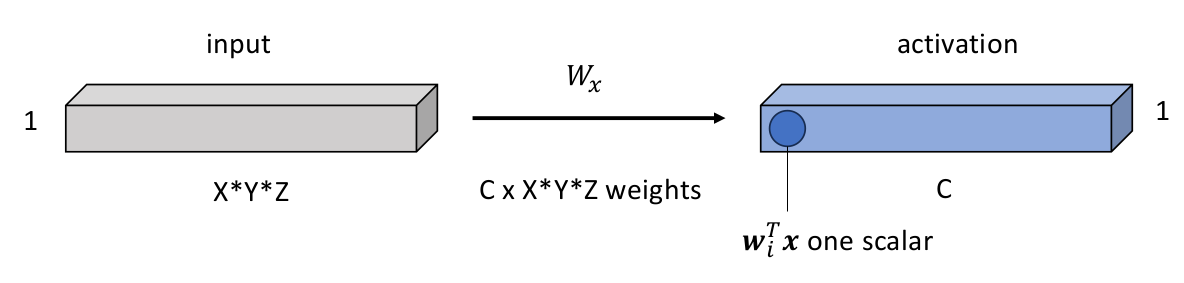
\includegraphics[width=\linewidth]{figures/input-tensor.png}
\end{figure}

In a typical Neural Network, you'd take an image with dimensions [X, Y, Z] for RGB channels and simply flatten it into a long vector of size XYZ x 1. This would then feed into the network for classification into C classes.

However, we have certain priors about image data that make this approach sub-optimal. Let's dive into these priors starting with the first principle: translation invariance. What we mean by this is that if you shift an object in an image, the intrinsic characteristics of the object don't change. Therefore, the features learned by the network should also shift accordingly. The second principle is locality. In image data, the relevant information for making a decision usually lies close to a particular location. It implies that we shouldn't have to scan the whole image to decide what a small region contains. In a fully connected network, this locality is not naturally accounted for, but in CNNs, it is. By keeping these principles in mind, Convolutional Neural Networks offer a more efficient and intuitively-aligned way to process image data compared to flattening the input as we would in conventional Neural Networks.

\begin{figure}[H]
    \centering
    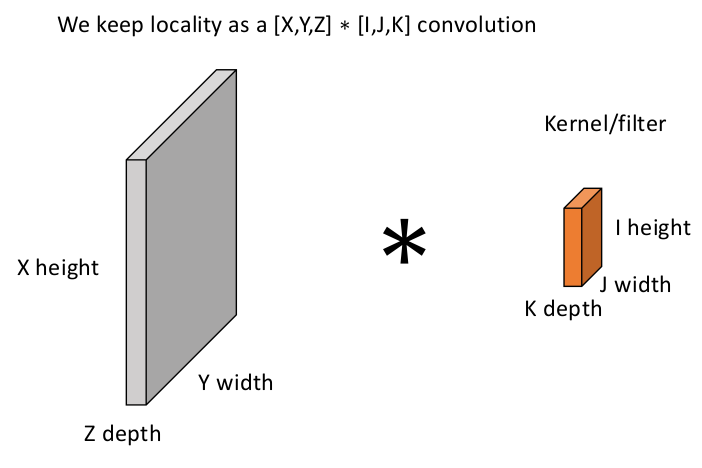
\includegraphics[width=.6\linewidth]{figures/Kernel.png}
\end{figure}

Instead of flattening the input image into a 1D vector as in a conventional Neural Network, CNNs maintain the original structure of the image as a 3D tensor of dimensions [X, Y, Z]. This helps us keep spatial relationships between pixels intact.

\subsection{Convolutional Layers}

This is the heart of a CNN, where filters or kernels slide across the input to produce feature maps. It captures local patterns and details like edges and textures, making it especially suited for image-related tasks.

\begin{figure}[H]
    \centering
    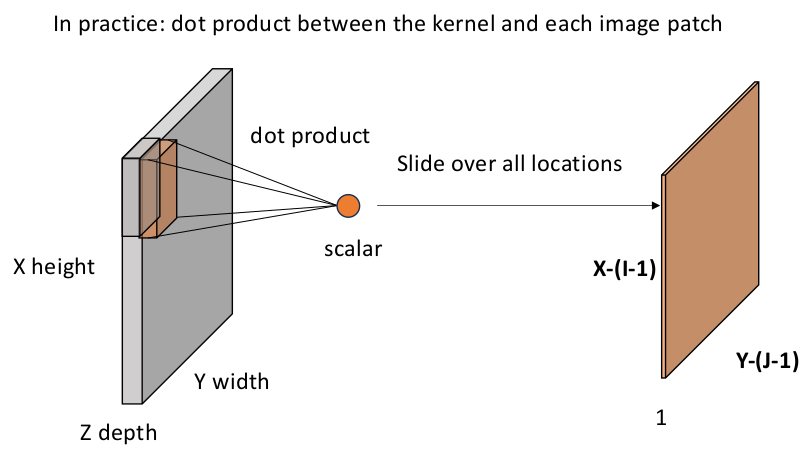
\includegraphics[width=.6\linewidth]{figures/convolution.png}
\end{figure}

This dot product is essentially a weighted sum of the pixel values in the image patch, where the weights are determined by the kernel. The output of each of these dot products forms a single pixel in the resulting feature map. This method is highly efficient and is one of the reasons why CNNs are so effective for image analysis tasks. It adheres to the principles of translation invariance and locality, capturing spatial features while significantly reducing the number of parameters compared to fully connected networks. 

To maintain the size of the image you can use zero-padding. Zero padding is the practice of adding zeros around the edge of the input image before applying the convolution operation. 

Preserving the dimensions of the input image can be beneficial for several reasons. For example, it allows for more layers to be stacked without shrinking the spatial dimensions too much, which can be particularly useful for deeper networks. By adding a border of zeros around the original input, you essentially create a buffer that allows the filter to slide across every position it would normally pass over if it could extend beyond the input's actual borders. This way, the output retains the same width and height dimensions as the input, ensuring that spatial relationships between features are maintained throughout the layers of the network.

\begin{figure}[H]
    \centering
    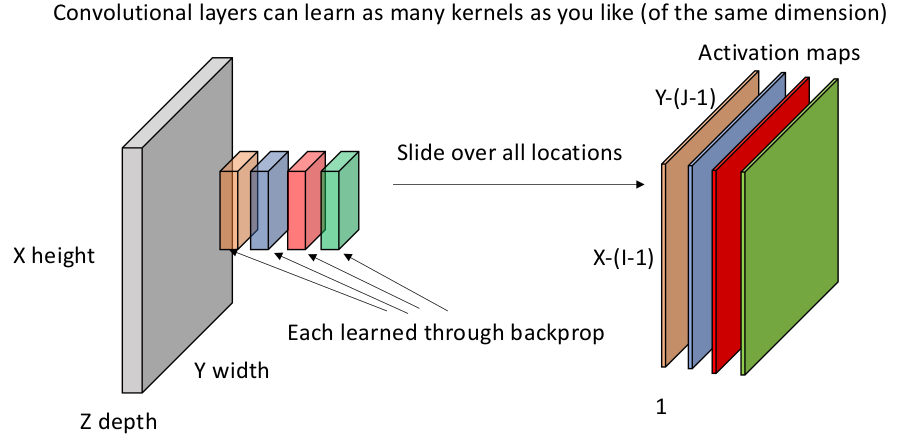
\includegraphics[width=.6\linewidth]{figures/features.png}
\end{figure}

convolutional layers can learn multiple filters, or kernels, at the same time, and all of them are of the same dimension. Why is this important? Each kernel captures a different feature or pattern in the input data. For example, one might specialize in detecting horizontal edges, while another might focus on capturing color gradients. Because these kernels are learned through back propagation, the network automatically adjusts them during training to capture the most important features for a given task. The images you see on the slide illustrate this concept. Each filter kernel has its own corresponding activation map, showing where in the image the particular feature it captures is located

\begin{figure}[H]
    \centering
    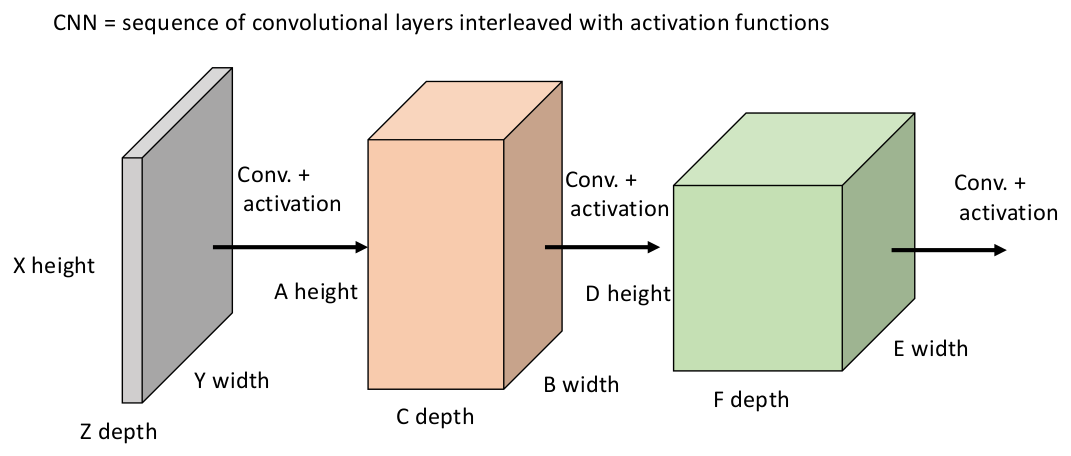
\includegraphics[width=.6\linewidth]{figures/CNN.png}
\end{figure}

At its core, a CNN is essentially a sequence of convolutional layers, each followed by an activation function. 

Each filter is defined by its dimensions: I, J, K. For a single filter, total number of parameters are $I\times J\times K + 1 (bias)$. The bias term is crucial because it allows the filter to have some flexibility, effectively shifting the activation function to better fit the data.

\subsection{1$\times$1 convolution}

\begin{figure}[H]
    \centering
    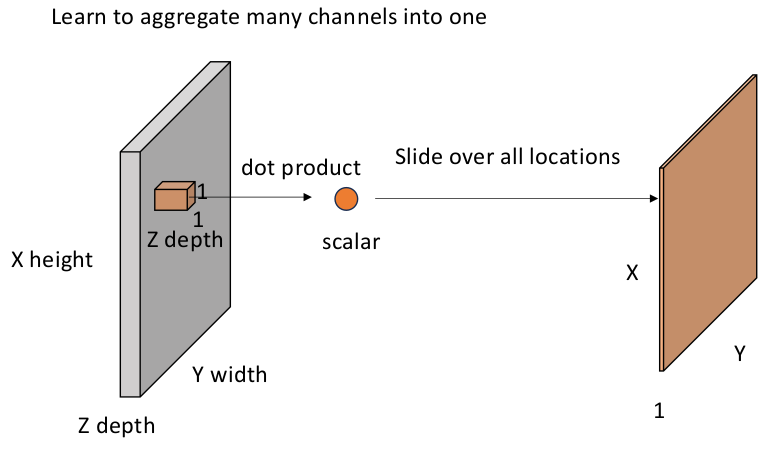
\includegraphics[width=.6\linewidth]{figures/reduction.png}
\end{figure}

The main utility of a 1x1 convolution is to reduce the depth of our network. Think of it as a way to perform dimensionality reduction across the depth of the feature map. When we have a high number of channels, or "depth", in our input volume, a 1x1 convolution can effectively condense that information. It's essentially a dot product operation across the depth of the input volume. As with regular convolutions, these 1x1 convolutions slide over all locations in the input. So, in a nutshell, 1x1 convolutions allow the network to learn how to aggregate many channels into fewer channels, thereby reducing computational complexity while maintaining important features.

\subsection{Factorized Convolutions}

\begin{figure}[H]
    \centering
    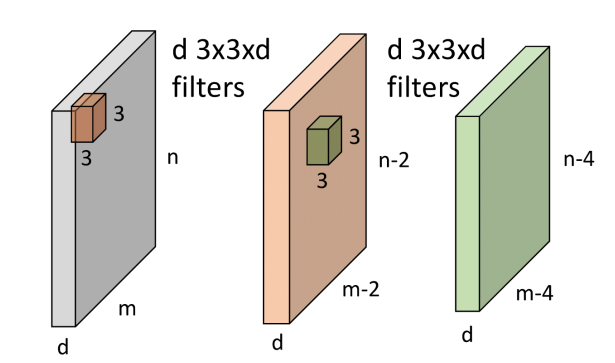
\includegraphics[width=.6\linewidth]{figures/factorized-convolutions.png}
\end{figure}

While two 3x3 convolutions might seem to serve as a good approximation for one 5x5 convolution, it's crucial to understand that this is indeed an approximation. You are essentially reducing the number of parameters and thus potentially the representational capacity of that layer. 

In a 5x5 convolution, you would typically have 25 parameters for each filter, excluding the bias term. When you break it down to two sequential 3x3 convolutions, each with 9 parameters, you end up with a total of 18 parameters, again excluding bias terms. 

The interesting trade-off here is between computational efficiency and expressiveness. Two 3x3 convolutions are computationally less expensive but may not capture the same level of detail as a single 5x5 convolution. 

Also, inserting an activation function between the two 3x3 convolutions introduces an extra non-linearity, making the approximation more capable of capturing complex features. However, this still doesn't match the 'possibilities' or parameter space offered by a single 5x5 filter. 

So when you opt for this factorization, remember that you're making a trade-off: gaining computational efficiency at the potential cost of some representational power.

\subsection{Separable Convolutions}

Separable convolutions aim to reduce the computational burden of this operation. Instead of a 5x5 convolution, you can approximate it by first applying a 1x5 convolution and then a 5x1 convolution. This breaks down the original 5x5 convolution into two separate operations, hence the name `separable'. 

Why is this useful? It's about computational efficiency. A single 5x5 convolution has 25 learnable parameters. But if you break it into a 1x5 followed by a 5x1 convolution, you have 5 parameters for the first convolution and 5 for the second, totalling 10 parameters. This effectively reduces the computational cost and also the number of learnable parameters, which can be very beneficial in large-scale or resource- constrained applications. 

However, it's crucial to note that this is an approximation technique. The catch is that it works well only if the original 5x5 filter can be accurately approximated by the two smaller filters. In some cases, this approximation might lead to a loss of information or representational power, but in practice, the efficiency gains often outweigh the drawbacks.

% \subsection{Activation Functions}

% Non-linearity is introduced here, allowing the model to learn complex mappings from inputs to outputs. ReLU, or Rectified Linear Unit, is commonly used because of its effectiveness in CNNs.

\subsection{Pooling Layers.}

This layer reduces the spatial dimensions of the feature maps, both simplifying the model and lessening the computational burden.  Max-pooling is often used as it retains the most salient features; Permutation-invariant aggregation+downsampling (typically max or avg)

\begin{enumerate}
    \item Reduces Resolution: Pooling makes the computational load lighter by reducing the     spatial dimensions.
    \item Hierarchical Features: As we progress through layers, pooling helps the network to     concentrate on increasingly abstract features, adding a level of hierarchy.
    \item Shift/Deformation Invariance: Pooling contributes to the network's robustness against    small shifts or deformations in the input.
\end{enumerate}

So, pooling is not just about making the network faster or lighter; it's a strategic component that adds robustness and translational invariance to the model.

\begin{figure}[H]
    \centering
    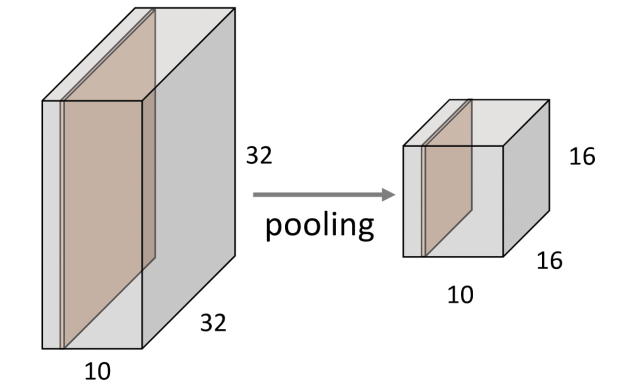
\includegraphics[width=.6\linewidth]{figures/pooling.png}
    \caption{Applied to each channel separately}
\end{figure}

\subsubsection{Max-pooling breaks shift-equivariance~\cite{youtubeMakingConvolutional}}

\begin{figure}
    \subfigure{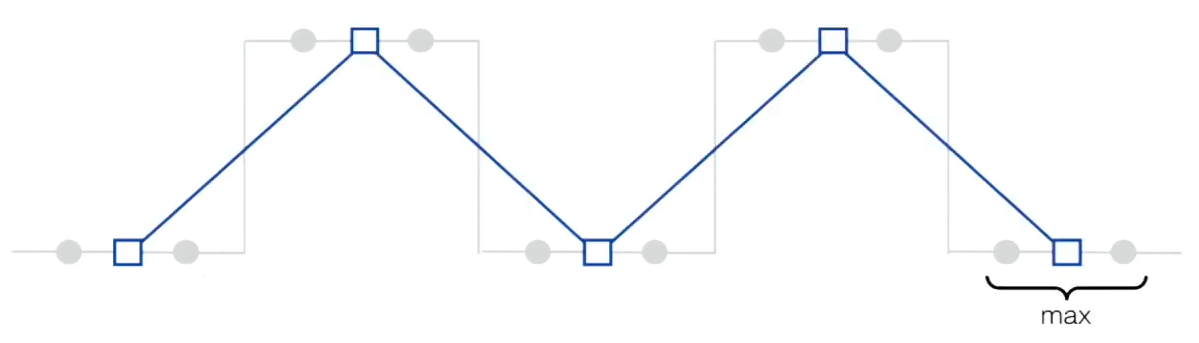
\includegraphics[width=\linewidth]{figures/max-pool-1.png}}
    \subfigure{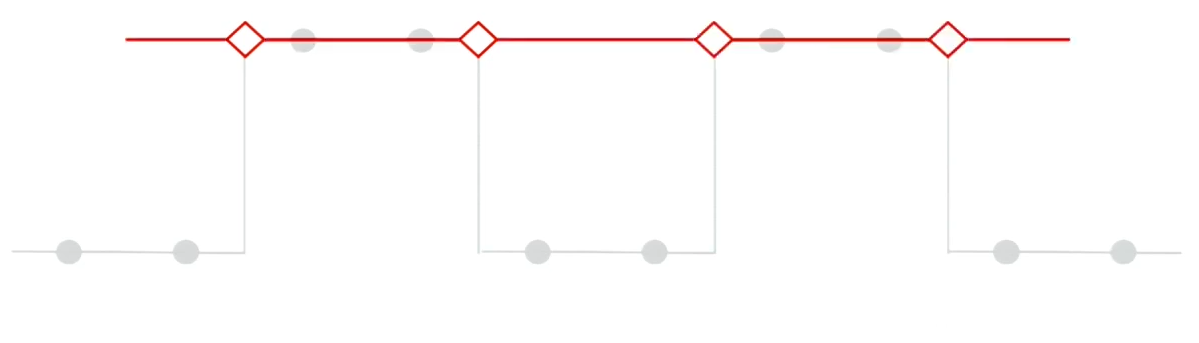
\includegraphics[width=\linewidth]{figures/max-pool-2.png}}
    \caption{Max-pooling breaks shift equivariance}
\end{figure}

Partial solution: use what you learned about anti-aliasing in Computer Vision: blur and then down sample

\subsection{Rotation?}

\begin{figure}[H]
    \centering
    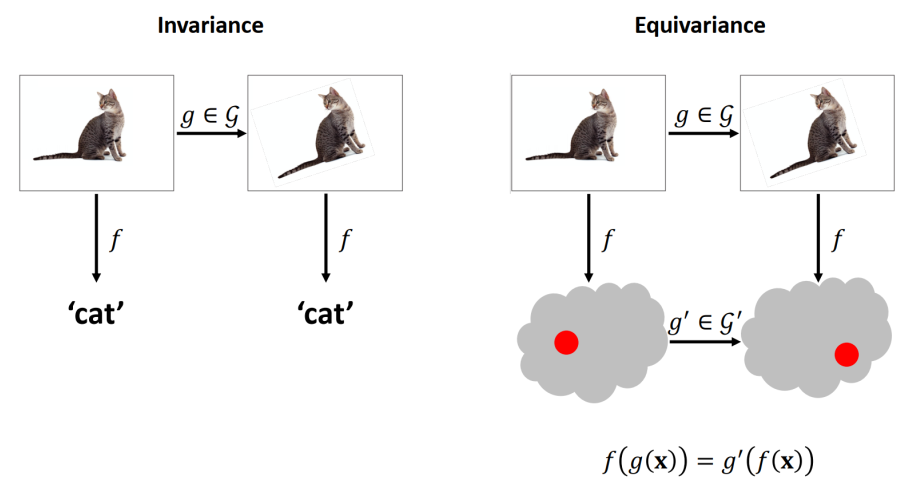
\includegraphics[width=.6\linewidth]{figures/cat-rotation.png}
\end{figure}

Unfortunately, standard CNNs are not naturally equivariant to rotations.

Before diving into how we can make CNNs rotation-equivariant, let's talk a bit about group theory. In mathematics, a group is a set of elements combined with an operation that is closed, meaning that combining two elements always results in another element from the same set. Rotations are a simple example of a group. If you rotate an object a bit to the left and then rotate it again, these two rotations can be combined into one effective rotation that achieves the same end result.

This leads us to Harmonic Networks or H-Nets. These are a specialized form of CNNs that are not just equivariant to translation but also to 360-degree rotations. This is achieved by replacing the standard filters in a CNN with what are called 'circular harmonics.' These specially designed filters ensure that a rotation in the input results in a proportionate rotation in the output feature maps, thus giving us rotation-equivariance.

\subsection{Approximate Deformation Invariance?}

CNNs can adapt to deformations or warping operations through a vector field $\tau$ which describes these shifts at a local level. However, one crucial factor that determines the success of CNNs in dealing with such deformations is how this vector field $\tau$ differs from a constant shift.

In a constant shift, every pixel moves by the same amount in the same direction. It's like moving a photograph sideways; every part of it moves uniformly. This is relatively easy for a CNN to handle due to its inherent translation invariance. However, in real-world scenarios, the shifts are often non-uniform; some pixels might move a lot, while others might barely move. These are described by a variable vector field $\tau$.

\begin{align*}
    \text{Digit 3 detector:} & f:\mathbb{R}^d \rightarrow \mathbb{R} \\
    \text{Wrap operator:} & D_\tau:\mathbb{R}^d \rightarrow \mathbb{R}^d & \text{wraping the image field by } \tau
\end{align*}

\begin{equation*}
    ||f(\vec{x})-f(D_\tau\vec{x})|| \approx || \triangledown \tau ||
\end{equation*}

% \subsection{Fully Connected Layers}

% Usually situated towards the end, this layer is where each neuron connects to every neuron in the previous layer, integrating the learned features for final predictions. 

\subsection{Flatten Layers}

This serves as a bridge between the convolutional layers and the fully connected layers, essentially converting 2D feature maps into 1D vectors.

\begin{figure}[H]
    \centering
    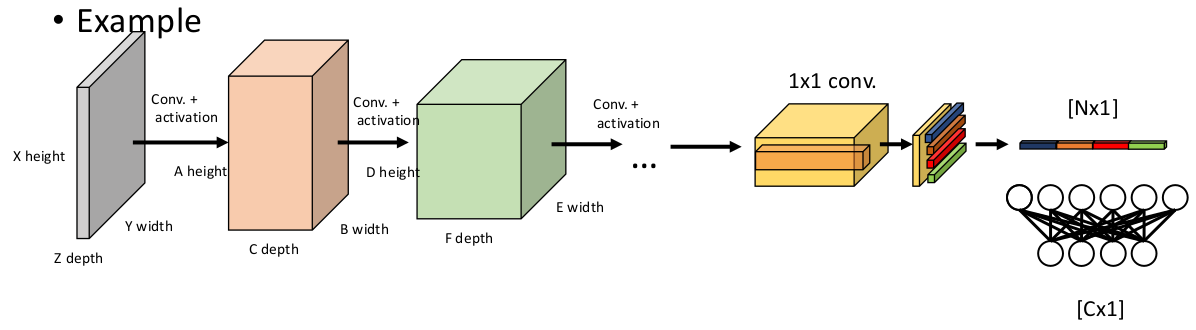
\includegraphics[width=\linewidth]{figures/flattening.png}
\end{figure}

Flattening layers serve as a connector between convolutional layers and fully connected layers in a Convolutional Neural Network (CNN). The flattening layer doesn't learn any parameters; it only reformats the data.

\subsection{Dimensions}

After padding and stride, the dimension of the image goes to:

\begin{equation}
    o= \lfloor \frac{i + 2p - k - (k-1)(d-1)}s \rfloor + 1
\end{equation}

Where

\begin{itemize}
    \item $i$ is the input size
    \item $p$ is the padding
    \item $k$ is the convolutional layer size
    \item $d$ is the dilation
    \item $s$ is the stride
\end{itemize}



\section{Conclusion}

\begin{enumerate}
    \item feature selection is important to build good representations. As we will
    see, the key of deep learning is to learn this feature selection instead of     doing it manually. 
    \item finding the right amount of features is key. Too few or too many will have a severe impact on the generalization abilities of your predictor model. Too few is easy too understand but too many requires an intuition about sample sparsity in high-dimensional spaces.
    \item the more features we choose as input the sparser our training samples will be distributed in the feature space. This means that decision boundaries become really tight around the used training samples because they all live close to each other at the boundaries of the space and our model will overfit the training data.
    \item weight sharing reduces the number of parameters from $n^2$ in a multi-layer perception to a small number, for example 3 as in our experiment or 3 by 3 image filter kernels or similar
    \item these filter kernels can be learned through back propagation exactly in the same way as you would train a multi-layer perception. Each layer may have many filter-kernels, so it will produce many filtered versions of the input with different filter functions.
    \item for real-valued functions, of a continuous or discrete variable, convolution differs from cross-correlation only in that either $f(x)$ or $g(x)$ is reflected about the y-axis; so it is a cross- correlation of $f(x)$ and $g(-x)$, or $f(-x)$ and $g(x)$.
    \item convolutions can massively reduce the computational complexity of neural networks but the real power of CNNs is revealed when priors are implemented and for example spatial structure is preserved. This is also one of the reasons why CNNs have been so successful in Computer Vision
    \item CNNs are pipeline of learnable filters interleaved with nonlinear activation functions producing d-dimensional feature maps at every stage. Training works like a common neural network: initialise randomly, present exampled from the training database, update the filter weights through backpropagation by propagating the error back through the network.
    \item convolution and pooling can be used to reduce the dimensionality of the input data until it forms a small enough representation space for either traditional machine learning methods for classification or regression or to steer other networks to for example generate a semantic interpretation like a mask of a particular object in the input.
\end{enumerate}
 
% \subsection{Dropout}

% This is a regularization technique that randomly deactivates a subset of neurons during training. This helps prevent overfitting and makes the network more robust.

% \subsection{Batch Normalization}

% This keeps the distribution of each layer's outputs stable, aiding in faster and more reliable training convergence.

 
\printbibliography

\end{document}